\documentclass[twoside]{book}

% Packages required by doxygen
\usepackage{fixltx2e}
\usepackage{calc}
\usepackage{doxygen}
\usepackage[export]{adjustbox} % also loads graphicx
\usepackage{graphicx}
\usepackage[utf8]{inputenc}
\usepackage{makeidx}
\usepackage{multicol}
\usepackage{multirow}
\PassOptionsToPackage{warn}{textcomp}
\usepackage{textcomp}
\usepackage[nointegrals]{wasysym}
\usepackage[table]{xcolor}

% Font selection
\usepackage[T1]{fontenc}
\usepackage[scaled=.90]{helvet}
\usepackage{courier}
\usepackage{amssymb}
\usepackage{sectsty}
\renewcommand{\familydefault}{\sfdefault}
\allsectionsfont{%
  \fontseries{bc}\selectfont%
  \color{darkgray}%
}
\renewcommand{\DoxyLabelFont}{%
  \fontseries{bc}\selectfont%
  \color{darkgray}%
}
\newcommand{\+}{\discretionary{\mbox{\scriptsize$\hookleftarrow$}}{}{}}

% Page & text layout
\usepackage{geometry}
\geometry{%
  a4paper,%
  top=2.5cm,%
  bottom=2.5cm,%
  left=2.5cm,%
  right=2.5cm%
}
\tolerance=750
\hfuzz=15pt
\hbadness=750
\setlength{\emergencystretch}{15pt}
\setlength{\parindent}{0cm}
\setlength{\parskip}{3ex plus 2ex minus 2ex}
\makeatletter
\renewcommand{\paragraph}{%
  \@startsection{paragraph}{4}{0ex}{-1.0ex}{1.0ex}{%
    \normalfont\normalsize\bfseries\SS@parafont%
  }%
}
\renewcommand{\subparagraph}{%
  \@startsection{subparagraph}{5}{0ex}{-1.0ex}{1.0ex}{%
    \normalfont\normalsize\bfseries\SS@subparafont%
  }%
}
\makeatother

% Headers & footers
\usepackage{fancyhdr}
\pagestyle{fancyplain}
\fancyhead[LE]{\fancyplain{}{\bfseries\thepage}}
\fancyhead[CE]{\fancyplain{}{}}
\fancyhead[RE]{\fancyplain{}{\bfseries\leftmark}}
\fancyhead[LO]{\fancyplain{}{\bfseries\rightmark}}
\fancyhead[CO]{\fancyplain{}{}}
\fancyhead[RO]{\fancyplain{}{\bfseries\thepage}}
\fancyfoot[LE]{\fancyplain{}{}}
\fancyfoot[CE]{\fancyplain{}{}}
\fancyfoot[RE]{\fancyplain{}{\bfseries\scriptsize Generated by Doxygen }}
\fancyfoot[LO]{\fancyplain{}{\bfseries\scriptsize Generated by Doxygen }}
\fancyfoot[CO]{\fancyplain{}{}}
\fancyfoot[RO]{\fancyplain{}{}}
\renewcommand{\footrulewidth}{0.4pt}
\renewcommand{\chaptermark}[1]{%
  \markboth{#1}{}%
}
\renewcommand{\sectionmark}[1]{%
  \markright{\thesection\ #1}%
}

% Indices & bibliography
\usepackage{natbib}
\usepackage[titles]{tocloft}
\setcounter{tocdepth}{3}
\setcounter{secnumdepth}{5}
\makeindex

% Hyperlinks (required, but should be loaded last)
\usepackage{ifpdf}
\ifpdf
  \usepackage[pdftex,pagebackref=true]{hyperref}
\else
  \usepackage[ps2pdf,pagebackref=true]{hyperref}
\fi
\hypersetup{%
  colorlinks=true,%
  linkcolor=blue,%
  citecolor=blue,%
  unicode%
}

% Custom commands
\newcommand{\clearemptydoublepage}{%
  \newpage{\pagestyle{empty}\cleardoublepage}%
}

\usepackage{caption}
\captionsetup{labelsep=space,justification=centering,font={bf},singlelinecheck=off,skip=4pt,position=top}

%===== C O N T E N T S =====

\begin{document}

% Titlepage & ToC
\hypersetup{pageanchor=false,
             bookmarksnumbered=true,
             pdfencoding=unicode
            }
\pagenumbering{alph}
\begin{titlepage}
\vspace*{7cm}
\begin{center}%
{\Large Computational Methods }\\
\vspace*{1cm}
{\large Generated by Doxygen 1.8.13}\\
\end{center}
\end{titlepage}
\clearemptydoublepage
\pagenumbering{roman}
\tableofcontents
\clearemptydoublepage
\pagenumbering{arabic}
\hypersetup{pageanchor=true}

%--- Begin generated contents ---
\chapter{Computational\+\_\+\+Methods}
\label{md__r_e_a_d_m_e}
\Hypertarget{md__r_e_a_d_m_e}
\input{md__r_e_a_d_m_e}
\chapter{Hierarchical Index}
\section{Class Hierarchy}
This inheritance list is sorted roughly, but not completely, alphabetically\+:\begin{DoxyCompactList}
\item \contentsline{section}{Output}{\pageref{class_output}}{}
\item \contentsline{section}{Solution}{\pageref{class_solution}}{}
\begin{DoxyCompactList}
\item \contentsline{section}{Analytical\+Solution}{\pageref{class_analytical_solution}}{}
\item \contentsline{section}{Crank\+Nicholson\+Method}{\pageref{class_crank_nicholson_method}}{}
\item \contentsline{section}{Du\+Fort\+Frankel\+Method}{\pageref{class_du_fort_frankel_method}}{}
\item \contentsline{section}{Laasonen\+Method}{\pageref{class_laasonen_method}}{}
\item \contentsline{section}{Richardson\+Method}{\pageref{class_richardson_method}}{}
\end{DoxyCompactList}
\item \contentsline{section}{Tools}{\pageref{class_tools}}{}
\end{DoxyCompactList}

\chapter{Class Index}
\section{Class List}
Here are the classes, structs, unions and interfaces with brief descriptions\+:\begin{DoxyCompactList}
\item\contentsline{section}{\hyperlink{class_matrix}{Matrix} }{\pageref{class_matrix}}{}
\item\contentsline{section}{\hyperlink{class_solution}{Solution} }{\pageref{class_solution}}{}
\item\contentsline{section}{\hyperlink{class_vector}{Vector} }{\pageref{class_vector}}{}
\end{DoxyCompactList}

\chapter{Class Documentation}
\hypertarget{class_matrix}{}\section{Matrix Class Reference}
\label{class_matrix}\index{Matrix@{Matrix}}


{\ttfamily \#include $<$matrix.\+h$>$}

Inheritance diagram for Matrix\+:\begin{figure}[H]
\begin{center}
\leavevmode
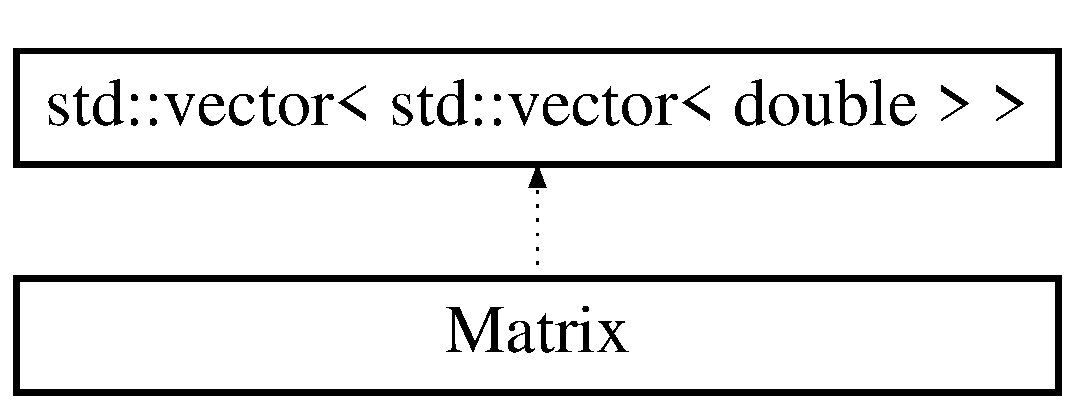
\includegraphics[height=2.000000cm]{class_matrix}
\end{center}
\end{figure}
\subsection*{Public Member Functions}
\begin{DoxyCompactItemize}
\item 
\hyperlink{class_matrix_a2dba13c45127354c9f75ef576f49269b}{Matrix} ()
\item 
\hyperlink{class_matrix_a135a15de1126d735bb95fcc839d739d7}{Matrix} (int Nrows, int Ncols)
\item 
\hyperlink{class_matrix_a765f4dcb51b6829311cc3e7576388423}{Matrix} (const \hyperlink{class_matrix}{Matrix} \&m)
\item 
int \hyperlink{class_matrix_a711f84a1c62832d9d197d78c9855a276}{get\+Nrows} () const
\item 
int \hyperlink{class_matrix_ae0a5f2154953b8d129a90b04f91d9079}{get\+Ncols} () const
\item 
\hyperlink{class_matrix}{Matrix} \& \hyperlink{class_matrix_aea5a06385f646eb4a63929fae6fa3e14}{operator=} (const \hyperlink{class_matrix}{Matrix} \&m)
\item 
bool \hyperlink{class_matrix_a35097c20bcb1495b57d452db0d7b1f53}{operator==} (const \hyperlink{class_matrix}{Matrix} \&m) const
\item 
double \hyperlink{class_matrix_af4d468252f3ecbbcaa5726c76e332b4c}{one\+\_\+norm} () const
\item 
double \hyperlink{class_matrix_aac496af05ec7aa26afc2b9c6d0ab8b66}{two\+\_\+norm} () const
\item 
double \hyperlink{class_matrix_a43066c7fe6418aad40170b85415063e8}{uniform\+\_\+norm} () const
\item 
\hyperlink{class_matrix}{Matrix} \hyperlink{class_matrix_aaa40c78e6b3bb5bbf572d35612dbf6a7}{operator$\ast$} (const \hyperlink{class_matrix}{Matrix} \&a) const
\item 
\hyperlink{class_vector}{Vector} \hyperlink{class_matrix_a843eebe2b6bd9d8091be600f685252cb}{operator$\ast$} (const \hyperlink{class_vector}{Vector} \&v) const
\item 
\hyperlink{class_matrix}{Matrix} \hyperlink{class_matrix_a759661b75b9681f3a89ff75e27933b3a}{transpose} () const
\end{DoxyCompactItemize}
\subsection*{Friends}
\begin{DoxyCompactItemize}
\item 
std\+::istream \& \hyperlink{class_matrix_a3d6c1dcfc038804f4c08687f4f37f48b}{operator$>$$>$} (std\+::istream \&is, \hyperlink{class_matrix}{Matrix} \&m)
\item 
std\+::ostream \& \hyperlink{class_matrix_a060711074cb5bcaf4e75498bc040c4b7}{operator$<$$<$} (std\+::ostream \&os, const \hyperlink{class_matrix}{Matrix} \&m)
\item 
std\+::ifstream \& \hyperlink{class_matrix_aa5699a0bdf0ee014f083ff8a76629d21}{operator$>$$>$} (std\+::ifstream \&ifs, \hyperlink{class_matrix}{Matrix} \&m)
\item 
std\+::ofstream \& \hyperlink{class_matrix_aa574249d63b390cf1108d6e82047ef61}{operator$<$$<$} (std\+::ofstream \&ofs, const \hyperlink{class_matrix}{Matrix} \&m)
\end{DoxyCompactItemize}


\subsection{Detailed Description}
A matrix class for data storage of a 2D array of doubles ~\newline
 The implementation is derived from the standard container vector std\+::vector ~\newline
 We use private inheritance to base our vector upon the library version whilst  usto expose only those base class functions we wish to use -\/ in this  the array access operator \mbox{[}\mbox{]}

The \hyperlink{class_matrix}{Matrix} class provides\+: ~\newline
-\/basic constructors for creating a matrix object from other matrix object,  by creating empty matrix of a given size, ~\newline
-\/input and oput operation via $>$$>$ and $<$$<$ operators using keyboard or file ~\newline
-\/basic operations like access via \mbox{[}\mbox{]} operator, assignment and comparision 

\subsection{Constructor \& Destructor Documentation}
\mbox{\Hypertarget{class_matrix_a2dba13c45127354c9f75ef576f49269b}\label{class_matrix_a2dba13c45127354c9f75ef576f49269b}} 
\index{Matrix@{Matrix}!Matrix@{Matrix}}
\index{Matrix@{Matrix}!Matrix@{Matrix}}
\subsubsection{\texorpdfstring{Matrix()}{Matrix()}\hspace{0.1cm}{\footnotesize\ttfamily [1/3]}}
{\footnotesize\ttfamily Matrix\+::\+Matrix (\begin{DoxyParamCaption}{ }\end{DoxyParamCaption})}

Default constructor. Intialize an empty \hyperlink{class_matrix}{Matrix} object \begin{DoxySeeAlso}{See also}
\hyperlink{class_matrix_a135a15de1126d735bb95fcc839d739d7}{Matrix(int Nrows, int Ncols)} 

\hyperlink{class_matrix_a765f4dcb51b6829311cc3e7576388423}{Matrix(const Matrix\& m)} 
\end{DoxySeeAlso}
\mbox{\Hypertarget{class_matrix_a135a15de1126d735bb95fcc839d739d7}\label{class_matrix_a135a15de1126d735bb95fcc839d739d7}} 
\index{Matrix@{Matrix}!Matrix@{Matrix}}
\index{Matrix@{Matrix}!Matrix@{Matrix}}
\subsubsection{\texorpdfstring{Matrix()}{Matrix()}\hspace{0.1cm}{\footnotesize\ttfamily [2/3]}}
{\footnotesize\ttfamily Matrix\+::\+Matrix (\begin{DoxyParamCaption}\item[{int}]{Nrows,  }\item[{int}]{Ncols }\end{DoxyParamCaption})}

Alternate constructor. build a matrix Nrows by Ncols \begin{DoxySeeAlso}{See also}
\hyperlink{class_matrix_a2dba13c45127354c9f75ef576f49269b}{Matrix()} 

\hyperlink{class_matrix_a765f4dcb51b6829311cc3e7576388423}{Matrix(const Matrix\& m)} 
\end{DoxySeeAlso}

\begin{DoxyExceptions}{Exceptions}
{\em invalid\+\_\+argument} & (\char`\"{}matrix size negative or zero\char`\"{}) \\
\hline
\end{DoxyExceptions}

\begin{DoxyParams}{Parameters}
{\em Nrows} & int. number of rows in matrix \\
\hline
{\em Ncols} & int. number of columns in matrix \\
\hline
\end{DoxyParams}
\mbox{\Hypertarget{class_matrix_a765f4dcb51b6829311cc3e7576388423}\label{class_matrix_a765f4dcb51b6829311cc3e7576388423}} 
\index{Matrix@{Matrix}!Matrix@{Matrix}}
\index{Matrix@{Matrix}!Matrix@{Matrix}}
\subsubsection{\texorpdfstring{Matrix()}{Matrix()}\hspace{0.1cm}{\footnotesize\ttfamily [3/3]}}
{\footnotesize\ttfamily Matrix\+::\+Matrix (\begin{DoxyParamCaption}\item[{const \hyperlink{class_matrix}{Matrix} \&}]{m }\end{DoxyParamCaption})}

Copy constructor. build a matrix from another matrix \begin{DoxySeeAlso}{See also}
\hyperlink{class_matrix_a2dba13c45127354c9f75ef576f49269b}{Matrix()} 

\hyperlink{class_matrix_a135a15de1126d735bb95fcc839d739d7}{Matrix(int Nrows, int Ncols)} 
\end{DoxySeeAlso}

\begin{DoxyParams}{Parameters}
{\em m} & \hyperlink{class_matrix}{Matrix}\&. matrix to copy from \\
\hline
\end{DoxyParams}


\subsection{Member Function Documentation}
\mbox{\Hypertarget{class_matrix_ae0a5f2154953b8d129a90b04f91d9079}\label{class_matrix_ae0a5f2154953b8d129a90b04f91d9079}} 
\index{Matrix@{Matrix}!get\+Ncols@{get\+Ncols}}
\index{get\+Ncols@{get\+Ncols}!Matrix@{Matrix}}
\subsubsection{\texorpdfstring{get\+Ncols()}{getNcols()}}
{\footnotesize\ttfamily int Matrix\+::get\+Ncols (\begin{DoxyParamCaption}{ }\end{DoxyParamCaption}) const}

Normal public get method. get the number of columns \begin{DoxySeeAlso}{See also}
int \hyperlink{class_matrix_a711f84a1c62832d9d197d78c9855a276}{get\+Nrows()const} 
\end{DoxySeeAlso}
\begin{DoxyReturn}{Returns}
int. number of columns in matrix 
\end{DoxyReturn}
\mbox{\Hypertarget{class_matrix_a711f84a1c62832d9d197d78c9855a276}\label{class_matrix_a711f84a1c62832d9d197d78c9855a276}} 
\index{Matrix@{Matrix}!get\+Nrows@{get\+Nrows}}
\index{get\+Nrows@{get\+Nrows}!Matrix@{Matrix}}
\subsubsection{\texorpdfstring{get\+Nrows()}{getNrows()}}
{\footnotesize\ttfamily int Matrix\+::get\+Nrows (\begin{DoxyParamCaption}{ }\end{DoxyParamCaption}) const}

Normal public get method. get the number of rows \begin{DoxySeeAlso}{See also}
int \hyperlink{class_matrix_ae0a5f2154953b8d129a90b04f91d9079}{get\+Ncols()const} 
\end{DoxySeeAlso}
\begin{DoxyReturn}{Returns}
int. number of rows in matrix 
\end{DoxyReturn}
\mbox{\Hypertarget{class_matrix_af4d468252f3ecbbcaa5726c76e332b4c}\label{class_matrix_af4d468252f3ecbbcaa5726c76e332b4c}} 
\index{Matrix@{Matrix}!one\+\_\+norm@{one\+\_\+norm}}
\index{one\+\_\+norm@{one\+\_\+norm}!Matrix@{Matrix}}
\subsubsection{\texorpdfstring{one\+\_\+norm()}{one\_norm()}}
{\footnotesize\ttfamily double Matrix\+::one\+\_\+norm (\begin{DoxyParamCaption}{ }\end{DoxyParamCaption}) const}

Normal public method that returns a double. It returns L1 norm of matrix \begin{DoxySeeAlso}{See also}
\hyperlink{class_matrix_aac496af05ec7aa26afc2b9c6d0ab8b66}{two\+\_\+norm()const} 

\hyperlink{class_matrix_a43066c7fe6418aad40170b85415063e8}{uniform\+\_\+norm()const} 
\end{DoxySeeAlso}
\begin{DoxyReturn}{Returns}
double. matrix L1 norm 
\end{DoxyReturn}
\mbox{\Hypertarget{class_matrix_aaa40c78e6b3bb5bbf572d35612dbf6a7}\label{class_matrix_aaa40c78e6b3bb5bbf572d35612dbf6a7}} 
\index{Matrix@{Matrix}!operator$\ast$@{operator$\ast$}}
\index{operator$\ast$@{operator$\ast$}!Matrix@{Matrix}}
\subsubsection{\texorpdfstring{operator$\ast$()}{operator*()}\hspace{0.1cm}{\footnotesize\ttfamily [1/2]}}
{\footnotesize\ttfamily \hyperlink{class_matrix}{Matrix} Matrix\+::operator$\ast$ (\begin{DoxyParamCaption}\item[{const \hyperlink{class_matrix}{Matrix} \&}]{a }\end{DoxyParamCaption}) const}

Overloaded $\ast$operator that returns a \hyperlink{class_matrix}{Matrix}. It Performs matrix by matrix multiplication. \begin{DoxySeeAlso}{See also}
\hyperlink{class_matrix_aaa40c78e6b3bb5bbf572d35612dbf6a7}{operator$\ast$(const Matrix \& a) const} 
\end{DoxySeeAlso}

\begin{DoxyExceptions}{Exceptions}
{\em out\+\_\+of\+\_\+range} & (\char`\"{}\+Matrix access error\char`\"{}) One or more of the matrix have a zero size \\
\hline
{\em std\+::out\+\_\+of\+\_\+range} & (\char`\"{}uncompatible matrix sizes\char`\"{}) Number of columns in first matrix do not match number of columns in second matrix \\
\hline
\end{DoxyExceptions}
\begin{DoxyReturn}{Returns}
\hyperlink{class_matrix}{Matrix}. matrix-\/matrix product 
\end{DoxyReturn}

\begin{DoxyParams}{Parameters}
{\em a} & \hyperlink{class_matrix}{Matrix}. matrix to multiply by \\
\hline
\end{DoxyParams}
\mbox{\Hypertarget{class_matrix_a843eebe2b6bd9d8091be600f685252cb}\label{class_matrix_a843eebe2b6bd9d8091be600f685252cb}} 
\index{Matrix@{Matrix}!operator$\ast$@{operator$\ast$}}
\index{operator$\ast$@{operator$\ast$}!Matrix@{Matrix}}
\subsubsection{\texorpdfstring{operator$\ast$()}{operator*()}\hspace{0.1cm}{\footnotesize\ttfamily [2/2]}}
{\footnotesize\ttfamily \hyperlink{class_vector}{Vector} Matrix\+::operator$\ast$ (\begin{DoxyParamCaption}\item[{const \hyperlink{class_vector}{Vector} \&}]{v }\end{DoxyParamCaption}) const}

Overloaded $\ast$operator that returns a \hyperlink{class_vector}{Vector}. It Performs matrix by vector multiplication. \begin{DoxySeeAlso}{See also}
\hyperlink{class_matrix_aaa40c78e6b3bb5bbf572d35612dbf6a7}{operator$\ast$(const Matrix \& a)const} 
\end{DoxySeeAlso}

\begin{DoxyExceptions}{Exceptions}
{\em std\+::out\+\_\+of\+\_\+range} & (\char`\"{}\+Matrix access error\char`\"{}) matrix has a zero size \\
\hline
{\em std\+::out\+\_\+of\+\_\+range} & (\char`\"{}\+Vector access error\char`\"{}) vector has a zero size \\
\hline
{\em std\+::out\+\_\+of\+\_\+range} & (\char`\"{}uncompatible matrix-\/vector sizes\char`\"{}) Number of columns in matrix do not match the vector size \\
\hline
\end{DoxyExceptions}
\begin{DoxyReturn}{Returns}
\hyperlink{class_vector}{Vector}. matrix-\/vector product 
\end{DoxyReturn}

\begin{DoxyParams}{Parameters}
{\em v} & \hyperlink{class_vector}{Vector}. \hyperlink{class_vector}{Vector} to multiply by \\
\hline
\end{DoxyParams}
\mbox{\Hypertarget{class_matrix_aea5a06385f646eb4a63929fae6fa3e14}\label{class_matrix_aea5a06385f646eb4a63929fae6fa3e14}} 
\index{Matrix@{Matrix}!operator=@{operator=}}
\index{operator=@{operator=}!Matrix@{Matrix}}
\subsubsection{\texorpdfstring{operator=()}{operator=()}}
{\footnotesize\ttfamily \hyperlink{class_matrix}{Matrix} \& Matrix\+::operator= (\begin{DoxyParamCaption}\item[{const \hyperlink{class_matrix}{Matrix} \&}]{m }\end{DoxyParamCaption})}

Overloaded assignment operator \begin{DoxySeeAlso}{See also}
\hyperlink{class_matrix_a35097c20bcb1495b57d452db0d7b1f53}{operator==(const Matrix\& m)const} 
\end{DoxySeeAlso}
\begin{DoxyReturn}{Returns}
\hyperlink{class_matrix}{Matrix}\&. the matrix on the left of the assignment 
\end{DoxyReturn}

\begin{DoxyParams}{Parameters}
{\em m} & \hyperlink{class_matrix}{Matrix}\&. \hyperlink{class_matrix}{Matrix} to assign from \\
\hline
\end{DoxyParams}
\mbox{\Hypertarget{class_matrix_a35097c20bcb1495b57d452db0d7b1f53}\label{class_matrix_a35097c20bcb1495b57d452db0d7b1f53}} 
\index{Matrix@{Matrix}!operator==@{operator==}}
\index{operator==@{operator==}!Matrix@{Matrix}}
\subsubsection{\texorpdfstring{operator==()}{operator==()}}
{\footnotesize\ttfamily bool Matrix\+::operator== (\begin{DoxyParamCaption}\item[{const \hyperlink{class_matrix}{Matrix} \&}]{m }\end{DoxyParamCaption}) const}

Overloaded comparison operator returns true or false depending on whether the matrices are the same or not \begin{DoxySeeAlso}{See also}
\hyperlink{class_matrix_aea5a06385f646eb4a63929fae6fa3e14}{operator=(const Matrix\& m)} 
\end{DoxySeeAlso}
\begin{DoxyReturn}{Returns}
bool. true or false 
\end{DoxyReturn}

\begin{DoxyParams}{Parameters}
{\em m} & \hyperlink{class_matrix}{Matrix}\&. \hyperlink{class_matrix}{Matrix} to compare to \\
\hline
\end{DoxyParams}
\mbox{\Hypertarget{class_matrix_a759661b75b9681f3a89ff75e27933b3a}\label{class_matrix_a759661b75b9681f3a89ff75e27933b3a}} 
\index{Matrix@{Matrix}!transpose@{transpose}}
\index{transpose@{transpose}!Matrix@{Matrix}}
\subsubsection{\texorpdfstring{transpose()}{transpose()}}
{\footnotesize\ttfamily \hyperlink{class_matrix}{Matrix} Matrix\+::transpose (\begin{DoxyParamCaption}{ }\end{DoxyParamCaption}) const}

public method that returns the transpose of the matrix. It returns the transpose of matrix \begin{DoxyReturn}{Returns}
\hyperlink{class_matrix}{Matrix}. matrix transpose 
\end{DoxyReturn}
\mbox{\Hypertarget{class_matrix_aac496af05ec7aa26afc2b9c6d0ab8b66}\label{class_matrix_aac496af05ec7aa26afc2b9c6d0ab8b66}} 
\index{Matrix@{Matrix}!two\+\_\+norm@{two\+\_\+norm}}
\index{two\+\_\+norm@{two\+\_\+norm}!Matrix@{Matrix}}
\subsubsection{\texorpdfstring{two\+\_\+norm()}{two\_norm()}}
{\footnotesize\ttfamily double Matrix\+::two\+\_\+norm (\begin{DoxyParamCaption}{ }\end{DoxyParamCaption}) const}

Normal public method that returns a double. It returns L2 norm of matrix \begin{DoxySeeAlso}{See also}
\hyperlink{class_matrix_af4d468252f3ecbbcaa5726c76e332b4c}{one\+\_\+norm()const} 

\hyperlink{class_matrix_a43066c7fe6418aad40170b85415063e8}{uniform\+\_\+norm()const} 
\end{DoxySeeAlso}
\begin{DoxyReturn}{Returns}
double. matrix L2 norm 
\end{DoxyReturn}
\mbox{\Hypertarget{class_matrix_a43066c7fe6418aad40170b85415063e8}\label{class_matrix_a43066c7fe6418aad40170b85415063e8}} 
\index{Matrix@{Matrix}!uniform\+\_\+norm@{uniform\+\_\+norm}}
\index{uniform\+\_\+norm@{uniform\+\_\+norm}!Matrix@{Matrix}}
\subsubsection{\texorpdfstring{uniform\+\_\+norm()}{uniform\_norm()}}
{\footnotesize\ttfamily double Matrix\+::uniform\+\_\+norm (\begin{DoxyParamCaption}{ }\end{DoxyParamCaption}) const}

Normal public method that returns a double. It returns L\+\_\+max norm of matrix \begin{DoxySeeAlso}{See also}
\hyperlink{class_matrix_af4d468252f3ecbbcaa5726c76e332b4c}{one\+\_\+norm()const} 

\hyperlink{class_matrix_aac496af05ec7aa26afc2b9c6d0ab8b66}{two\+\_\+norm()const} 
\end{DoxySeeAlso}
\begin{DoxyReturn}{Returns}
double. matrix L\+\_\+max norm 
\end{DoxyReturn}


\subsection{Friends And Related Function Documentation}
\mbox{\Hypertarget{class_matrix_a060711074cb5bcaf4e75498bc040c4b7}\label{class_matrix_a060711074cb5bcaf4e75498bc040c4b7}} 
\index{Matrix@{Matrix}!operator$<$$<$@{operator$<$$<$}}
\index{operator$<$$<$@{operator$<$$<$}!Matrix@{Matrix}}
\subsubsection{\texorpdfstring{operator$<$$<$}{operator<<}\hspace{0.1cm}{\footnotesize\ttfamily [1/2]}}
{\footnotesize\ttfamily std\+::ostream\& operator$<$$<$ (\begin{DoxyParamCaption}\item[{std\+::ostream \&}]{os,  }\item[{const \hyperlink{class_matrix}{Matrix} \&}]{m }\end{DoxyParamCaption})\hspace{0.3cm}{\ttfamily [friend]}}

Overloaded ostream $<$$<$ operator. Display output if matrix has size user will be asked to input only matrix values if matrix was not initialized user can choose matrix size and input it values \begin{DoxySeeAlso}{See also}
\hyperlink{class_matrix_aa5699a0bdf0ee014f083ff8a76629d21}{operator$>$$>$(std\+::ifstream\& ifs, Matrix\& m)} 

\hyperlink{class_matrix_a3d6c1dcfc038804f4c08687f4f37f48b}{operator$>$$>$(std\+::istream\& is, Matrix\& m)} 

\hyperlink{class_matrix_a060711074cb5bcaf4e75498bc040c4b7}{operator$<$$<$(std\+::ostream\& os, const Matrix\& m)} 
\end{DoxySeeAlso}
\begin{DoxyReturn}{Returns}
std\+::ostream\&. The ostream object 
\end{DoxyReturn}

\begin{DoxyParams}{Parameters}
{\em os} & Display output stream \\
\hline
{\em m} & \hyperlink{class_matrix}{Matrix} to read from \\
\hline
\end{DoxyParams}
\mbox{\Hypertarget{class_matrix_aa574249d63b390cf1108d6e82047ef61}\label{class_matrix_aa574249d63b390cf1108d6e82047ef61}} 
\index{Matrix@{Matrix}!operator$<$$<$@{operator$<$$<$}}
\index{operator$<$$<$@{operator$<$$<$}!Matrix@{Matrix}}
\subsubsection{\texorpdfstring{operator$<$$<$}{operator<<}\hspace{0.1cm}{\footnotesize\ttfamily [2/2]}}
{\footnotesize\ttfamily std\+::ofstream\& operator$<$$<$ (\begin{DoxyParamCaption}\item[{std\+::ofstream \&}]{ofs,  }\item[{const \hyperlink{class_matrix}{Matrix} \&}]{m }\end{DoxyParamCaption})\hspace{0.3cm}{\ttfamily [friend]}}

Overloaded ofstream $<$$<$ operator. File output the file output operator is compatible with file input operator, ie. everything written can be read later. \begin{DoxySeeAlso}{See also}
\hyperlink{class_matrix_aa5699a0bdf0ee014f083ff8a76629d21}{operator$>$$>$(std\+::ifstream\& ifs, Matrix\& m)} 

\hyperlink{class_matrix_aa574249d63b390cf1108d6e82047ef61}{operator$<$$<$(std\+::ofstream\& ofs, const Matrix\& m)} 

\hyperlink{class_matrix_a3d6c1dcfc038804f4c08687f4f37f48b}{operator$>$$>$(std\+::istream\& is, Matrix\& m)} 
\end{DoxySeeAlso}

\begin{DoxyExceptions}{Exceptions}
{\em std\+::invalid\+\_\+argument} & (\char`\"{}file read error -\/ negative matrix size\char`\"{}); \\
\hline
\end{DoxyExceptions}
\begin{DoxyReturn}{Returns}
std\+::ofstream\&. The ofstream object 
\end{DoxyReturn}

\begin{DoxyParams}{Parameters}
{\em m} & \hyperlink{class_matrix}{Matrix} to read from \\
\hline
\end{DoxyParams}
\mbox{\Hypertarget{class_matrix_a3d6c1dcfc038804f4c08687f4f37f48b}\label{class_matrix_a3d6c1dcfc038804f4c08687f4f37f48b}} 
\index{Matrix@{Matrix}!operator$>$$>$@{operator$>$$>$}}
\index{operator$>$$>$@{operator$>$$>$}!Matrix@{Matrix}}
\subsubsection{\texorpdfstring{operator$>$$>$}{operator>>}\hspace{0.1cm}{\footnotesize\ttfamily [1/2]}}
{\footnotesize\ttfamily std\+::istream\& operator$>$$>$ (\begin{DoxyParamCaption}\item[{std\+::istream \&}]{is,  }\item[{\hyperlink{class_matrix}{Matrix} \&}]{m }\end{DoxyParamCaption})\hspace{0.3cm}{\ttfamily [friend]}}

Overloaded istream $>$$>$ operator. Keyboard input if matrix has size user will be asked to input only matrix values if matrix was not initialized user can choose matrix size and input it values \begin{DoxySeeAlso}{See also}
\hyperlink{class_matrix_aa574249d63b390cf1108d6e82047ef61}{operator$<$$<$(std\+::ofstream\& ofs, const Matrix\& m)} 

\hyperlink{class_matrix_a3d6c1dcfc038804f4c08687f4f37f48b}{operator$>$$>$(std\+::istream\& is, Matrix\& m)} 

\hyperlink{class_matrix_a060711074cb5bcaf4e75498bc040c4b7}{operator$<$$<$(std\+::ostream\& os, const Matrix\& m)} 
\end{DoxySeeAlso}

\begin{DoxyExceptions}{Exceptions}
{\em std\+::invalid\+\_\+argument} & (\char`\"{}read error -\/ negative matrix size\char`\"{}); \\
\hline
\end{DoxyExceptions}
\begin{DoxyReturn}{Returns}
std\+::istream\&. The istream object 
\end{DoxyReturn}

\begin{DoxyParams}{Parameters}
{\em is} & Keyboard input stream \\
\hline
{\em m} & \hyperlink{class_matrix}{Matrix} to write into \\
\hline
\end{DoxyParams}
\mbox{\Hypertarget{class_matrix_aa5699a0bdf0ee014f083ff8a76629d21}\label{class_matrix_aa5699a0bdf0ee014f083ff8a76629d21}} 
\index{Matrix@{Matrix}!operator$>$$>$@{operator$>$$>$}}
\index{operator$>$$>$@{operator$>$$>$}!Matrix@{Matrix}}
\subsubsection{\texorpdfstring{operator$>$$>$}{operator>>}\hspace{0.1cm}{\footnotesize\ttfamily [2/2]}}
{\footnotesize\ttfamily std\+::ifstream\& operator$>$$>$ (\begin{DoxyParamCaption}\item[{std\+::ifstream \&}]{ifs,  }\item[{\hyperlink{class_matrix}{Matrix} \&}]{m }\end{DoxyParamCaption})\hspace{0.3cm}{\ttfamily [friend]}}

Overloaded ifstream $>$$>$ operator. File input the file output operator is compatible with file input operator, ie. everything written can be read later. \begin{DoxySeeAlso}{See also}
\hyperlink{class_matrix_aa5699a0bdf0ee014f083ff8a76629d21}{operator$>$$>$(std\+::ifstream\& ifs, Matrix\& m)} 

\hyperlink{class_matrix_aa574249d63b390cf1108d6e82047ef61}{operator$<$$<$(std\+::ofstream\& ofs, const Matrix\& m)} 

\hyperlink{class_matrix_a060711074cb5bcaf4e75498bc040c4b7}{operator$<$$<$(std\+::ostream\& os, const Matrix\& m)} 
\end{DoxySeeAlso}
\begin{DoxyReturn}{Returns}
std\+::ifstream\&. The ifstream object 
\end{DoxyReturn}

\begin{DoxyParams}{Parameters}
{\em ifs} & Input file stream with opened matrix file \\
\hline
{\em m} & \hyperlink{class_matrix}{Matrix} to write into \\
\hline
\end{DoxyParams}


The documentation for this class was generated from the following files\+:\begin{DoxyCompactItemize}
\item 
matrix.\+h\item 
matrix.\+cpp\end{DoxyCompactItemize}

\hypertarget{class_vector}{}\section{Vector Class Reference}
\label{class_vector}\index{Vector@{Vector}}


{\ttfamily \#include $<$vector.\+h$>$}

Inheritance diagram for Vector\+:\begin{figure}[H]
\begin{center}
\leavevmode
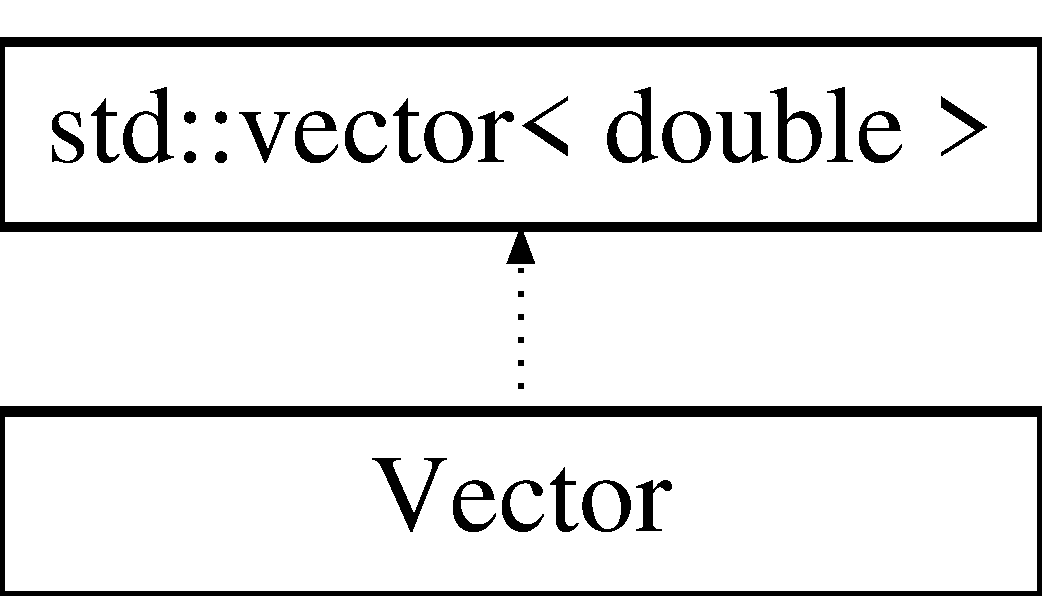
\includegraphics[height=2.000000cm]{class_vector}
\end{center}
\end{figure}
\subsection*{Public Member Functions}
\begin{DoxyCompactItemize}
\item 
\hyperlink{class_vector_a6f80c73b5f18dcf3f8e36065bdc8b9e5}{Vector} ()
\item 
\hyperlink{class_vector_acbdf66550f2caa0a64e0b356fb63a277}{Vector} (int Num)
\item 
\hyperlink{class_vector_a5f04e343b7306ad11f8a82c89b486764}{Vector} (const \hyperlink{class_vector}{Vector} \&v)
\item 
\hyperlink{class_vector}{Vector} \& \hyperlink{class_vector_ae48c467a9f65d60e2f7455aba4ca1239}{operator=} (const \hyperlink{class_vector}{Vector} \&v)
\item 
bool \hyperlink{class_vector_ade5fbd0cd01b034d1907e0c93433320c}{operator==} (const \hyperlink{class_vector}{Vector} \&v) const
\item 
int \hyperlink{class_vector_afbb7966ec4107c43ec15cccc47fcaef7}{get\+Size} () const
\item 
double \hyperlink{class_vector_a6752a90058ddef427ca6aed12946a737}{one\+\_\+norm} () const
\item 
double \hyperlink{class_vector_a4f501290a50d057bb6c57ea64d7e70a4}{two\+\_\+norm} () const
\item 
double \hyperlink{class_vector_a50b72131eaf3698a9876d99ab6912a32}{uniform\+\_\+norm} () const
\end{DoxyCompactItemize}
\subsection*{Friends}
\begin{DoxyCompactItemize}
\item 
std\+::istream \& \hyperlink{class_vector_ac198cff0f4196c66649278458eebf227}{operator$>$$>$} (std\+::istream \&is, \hyperlink{class_vector}{Vector} \&v)
\item 
std\+::ostream \& \hyperlink{class_vector_ac254b27efeb8486ee2f67821e3a21a60}{operator$<$$<$} (std\+::ostream \&os, const \hyperlink{class_vector}{Vector} \&v)
\item 
std\+::ifstream \& \hyperlink{class_vector_ab6009b37fac65598b3db164dc4f19fed}{operator$>$$>$} (std\+::ifstream \&ifs, \hyperlink{class_vector}{Vector} \&v)
\item 
std\+::ofstream \& \hyperlink{class_vector_a8e755f5550c983df730602890058d990}{operator$<$$<$} (std\+::ofstream \&ofs, const \hyperlink{class_vector}{Vector} \&v)
\end{DoxyCompactItemize}


\subsection{Detailed Description}
A vector class for data storage of a 1D array of doubles ~\newline
 The implementation is derived from the standard container vector std\+::vector ~\newline
 We use private inheritance to base our vector upon the library version whilst  usto expose only those base class functions we wish to use -\/ in this  the array access operator \mbox{[}\mbox{]}

The \hyperlink{class_vector}{Vector} class provides\+: ~\newline
-\/basic constructors for creating vector obcjet from other vector object, or by creating empty vector of a given size, ~\newline
-\/input and oput operation via $>$$>$ and $<$$<$ operators using keyboard or file ~\newline
-\/basic operations like access via \mbox{[}\mbox{]} operator, assignment and comparision 

\subsection{Constructor \& Destructor Documentation}
\mbox{\Hypertarget{class_vector_a6f80c73b5f18dcf3f8e36065bdc8b9e5}\label{class_vector_a6f80c73b5f18dcf3f8e36065bdc8b9e5}} 
\index{Vector@{Vector}!Vector@{Vector}}
\index{Vector@{Vector}!Vector@{Vector}}
\subsubsection{\texorpdfstring{Vector()}{Vector()}\hspace{0.1cm}{\footnotesize\ttfamily [1/3]}}
{\footnotesize\ttfamily Vector\+::\+Vector (\begin{DoxyParamCaption}{ }\end{DoxyParamCaption})}

Default constructor. Intialize an empty \hyperlink{class_vector}{Vector} object \begin{DoxySeeAlso}{See also}
\hyperlink{class_vector_acbdf66550f2caa0a64e0b356fb63a277}{Vector(int Num)} 

\hyperlink{class_vector_a5f04e343b7306ad11f8a82c89b486764}{Vector(const Vector\& v)} 
\end{DoxySeeAlso}
\mbox{\Hypertarget{class_vector_acbdf66550f2caa0a64e0b356fb63a277}\label{class_vector_acbdf66550f2caa0a64e0b356fb63a277}} 
\index{Vector@{Vector}!Vector@{Vector}}
\index{Vector@{Vector}!Vector@{Vector}}
\subsubsection{\texorpdfstring{Vector()}{Vector()}\hspace{0.1cm}{\footnotesize\ttfamily [2/3]}}
{\footnotesize\ttfamily Vector\+::\+Vector (\begin{DoxyParamCaption}\item[{int}]{Num }\end{DoxyParamCaption})\hspace{0.3cm}{\ttfamily [explicit]}}

Explicit alterative constructor takes an intiger. it is explicit since implicit type conversion int -\/$>$ vector doesn\textquotesingle{}t make sense Intialize \hyperlink{class_vector}{Vector} object of size Num \begin{DoxySeeAlso}{See also}
\hyperlink{class_vector_a6f80c73b5f18dcf3f8e36065bdc8b9e5}{Vector()} 

\hyperlink{class_vector_a5f04e343b7306ad11f8a82c89b486764}{Vector(const Vector\& v)} 
\end{DoxySeeAlso}

\begin{DoxyExceptions}{Exceptions}
{\em invalid\+\_\+argument} & (\char`\"{}vector size negative\char`\"{}) \\
\hline
\end{DoxyExceptions}

\begin{DoxyParams}{Parameters}
{\em Num} & int. Size of a vector \\
\hline
\end{DoxyParams}
\mbox{\Hypertarget{class_vector_a5f04e343b7306ad11f8a82c89b486764}\label{class_vector_a5f04e343b7306ad11f8a82c89b486764}} 
\index{Vector@{Vector}!Vector@{Vector}}
\index{Vector@{Vector}!Vector@{Vector}}
\subsubsection{\texorpdfstring{Vector()}{Vector()}\hspace{0.1cm}{\footnotesize\ttfamily [3/3]}}
{\footnotesize\ttfamily Vector\+::\+Vector (\begin{DoxyParamCaption}\item[{const \hyperlink{class_vector}{Vector} \&}]{v }\end{DoxyParamCaption})}

Copy constructor takes an \hyperlink{class_vector}{Vector} object reference. Intialize \hyperlink{class_vector}{Vector} object with another \hyperlink{class_vector}{Vector} object \begin{DoxySeeAlso}{See also}
\hyperlink{class_vector_a6f80c73b5f18dcf3f8e36065bdc8b9e5}{Vector()} 

\hyperlink{class_vector_acbdf66550f2caa0a64e0b356fb63a277}{Vector(int Num)} 
\end{DoxySeeAlso}


\subsection{Member Function Documentation}
\mbox{\Hypertarget{class_vector_afbb7966ec4107c43ec15cccc47fcaef7}\label{class_vector_afbb7966ec4107c43ec15cccc47fcaef7}} 
\index{Vector@{Vector}!get\+Size@{get\+Size}}
\index{get\+Size@{get\+Size}!Vector@{Vector}}
\subsubsection{\texorpdfstring{get\+Size()}{getSize()}}
{\footnotesize\ttfamily int Vector\+::get\+Size (\begin{DoxyParamCaption}{ }\end{DoxyParamCaption}) const}

Normal get method that returns integer, the size of the vector \begin{DoxyReturn}{Returns}
int. the size of the vector 
\end{DoxyReturn}
\mbox{\Hypertarget{class_vector_a6752a90058ddef427ca6aed12946a737}\label{class_vector_a6752a90058ddef427ca6aed12946a737}} 
\index{Vector@{Vector}!one\+\_\+norm@{one\+\_\+norm}}
\index{one\+\_\+norm@{one\+\_\+norm}!Vector@{Vector}}
\subsubsection{\texorpdfstring{one\+\_\+norm()}{one\_norm()}}
{\footnotesize\ttfamily double Vector\+::one\+\_\+norm (\begin{DoxyParamCaption}{ }\end{DoxyParamCaption}) const}

Normal public method that returns a double. It returns L1 norm of vector \begin{DoxySeeAlso}{See also}
\hyperlink{class_vector_a4f501290a50d057bb6c57ea64d7e70a4}{two\+\_\+norm()const} 

\hyperlink{class_vector_a50b72131eaf3698a9876d99ab6912a32}{uniform\+\_\+norm()const} 
\end{DoxySeeAlso}
\begin{DoxyReturn}{Returns}
double. vectors L1 norm 
\end{DoxyReturn}
\mbox{\Hypertarget{class_vector_ae48c467a9f65d60e2f7455aba4ca1239}\label{class_vector_ae48c467a9f65d60e2f7455aba4ca1239}} 
\index{Vector@{Vector}!operator=@{operator=}}
\index{operator=@{operator=}!Vector@{Vector}}
\subsubsection{\texorpdfstring{operator=()}{operator=()}}
{\footnotesize\ttfamily \hyperlink{class_vector}{Vector} \& Vector\+::operator= (\begin{DoxyParamCaption}\item[{const \hyperlink{class_vector}{Vector} \&}]{v }\end{DoxyParamCaption})}

Overloaded assignment operator \begin{DoxySeeAlso}{See also}
\hyperlink{class_vector_ade5fbd0cd01b034d1907e0c93433320c}{operator==(const Vector\& v)const} 
\end{DoxySeeAlso}

\begin{DoxyParams}{Parameters}
{\em v} & \hyperlink{class_vector}{Vector} to assign from \\
\hline
\end{DoxyParams}
\begin{DoxyReturn}{Returns}
the object on the left of the assignment 
\end{DoxyReturn}

\begin{DoxyParams}{Parameters}
{\em v} & Vecto\&. \hyperlink{class_vector}{Vector} to assign from \\
\hline
\end{DoxyParams}
\mbox{\Hypertarget{class_vector_ade5fbd0cd01b034d1907e0c93433320c}\label{class_vector_ade5fbd0cd01b034d1907e0c93433320c}} 
\index{Vector@{Vector}!operator==@{operator==}}
\index{operator==@{operator==}!Vector@{Vector}}
\subsubsection{\texorpdfstring{operator==()}{operator==()}}
{\footnotesize\ttfamily bool Vector\+::operator== (\begin{DoxyParamCaption}\item[{const \hyperlink{class_vector}{Vector} \&}]{v }\end{DoxyParamCaption}) const}

Overloaded comparison operator returns true if vectors are the same within a tolerance (1.\+e-\/07) \begin{DoxySeeAlso}{See also}
\hyperlink{class_vector_ae48c467a9f65d60e2f7455aba4ca1239}{operator=(const Vector\& v)} 

operator\mbox{[}$\,$\mbox{]}(int i) 

operator\mbox{[}$\,$\mbox{]}(int i)const 
\end{DoxySeeAlso}
\begin{DoxyReturn}{Returns}
bool. true or false 
\end{DoxyReturn}

\begin{DoxyExceptions}{Exceptions}
{\em invalid\+\_\+argument} & (\char`\"{}incompatible vector sizes\textbackslash{}n\char`\"{}) \\
\hline
\end{DoxyExceptions}

\begin{DoxyParams}{Parameters}
{\em v} & \hyperlink{class_vector}{Vector}\&. vector to compare \\
\hline
\end{DoxyParams}
\mbox{\Hypertarget{class_vector_a4f501290a50d057bb6c57ea64d7e70a4}\label{class_vector_a4f501290a50d057bb6c57ea64d7e70a4}} 
\index{Vector@{Vector}!two\+\_\+norm@{two\+\_\+norm}}
\index{two\+\_\+norm@{two\+\_\+norm}!Vector@{Vector}}
\subsubsection{\texorpdfstring{two\+\_\+norm()}{two\_norm()}}
{\footnotesize\ttfamily double Vector\+::two\+\_\+norm (\begin{DoxyParamCaption}{ }\end{DoxyParamCaption}) const}

Normal public method that returns a double. It returns L2 norm of vector \begin{DoxySeeAlso}{See also}
\hyperlink{class_vector_a6752a90058ddef427ca6aed12946a737}{one\+\_\+norm()const} 

\hyperlink{class_vector_a50b72131eaf3698a9876d99ab6912a32}{uniform\+\_\+norm()const} 
\end{DoxySeeAlso}
\begin{DoxyReturn}{Returns}
double. vectors L2 norm 
\end{DoxyReturn}
\mbox{\Hypertarget{class_vector_a50b72131eaf3698a9876d99ab6912a32}\label{class_vector_a50b72131eaf3698a9876d99ab6912a32}} 
\index{Vector@{Vector}!uniform\+\_\+norm@{uniform\+\_\+norm}}
\index{uniform\+\_\+norm@{uniform\+\_\+norm}!Vector@{Vector}}
\subsubsection{\texorpdfstring{uniform\+\_\+norm()}{uniform\_norm()}}
{\footnotesize\ttfamily double Vector\+::uniform\+\_\+norm (\begin{DoxyParamCaption}{ }\end{DoxyParamCaption}) const}

Normal public method that returns a double. It returns L\+\_\+max norm of vector \begin{DoxySeeAlso}{See also}
\hyperlink{class_vector_a6752a90058ddef427ca6aed12946a737}{one\+\_\+norm()const} 

\hyperlink{class_vector_a4f501290a50d057bb6c57ea64d7e70a4}{two\+\_\+norm()const} 
\end{DoxySeeAlso}

\begin{DoxyExceptions}{Exceptions}
{\em out\+\_\+of\+\_\+range} & (\char`\"{}vector access error\char`\"{}) vector has zero size \\
\hline
\end{DoxyExceptions}
\begin{DoxyReturn}{Returns}
double. vectors Lmax norm 
\end{DoxyReturn}


\subsection{Friends And Related Function Documentation}
\mbox{\Hypertarget{class_vector_ac254b27efeb8486ee2f67821e3a21a60}\label{class_vector_ac254b27efeb8486ee2f67821e3a21a60}} 
\index{Vector@{Vector}!operator$<$$<$@{operator$<$$<$}}
\index{operator$<$$<$@{operator$<$$<$}!Vector@{Vector}}
\subsubsection{\texorpdfstring{operator$<$$<$}{operator<<}\hspace{0.1cm}{\footnotesize\ttfamily [1/2]}}
{\footnotesize\ttfamily std\+::ostream\& operator$<$$<$ (\begin{DoxyParamCaption}\item[{std\+::ostream \&}]{os,  }\item[{const \hyperlink{class_vector}{Vector} \&}]{v }\end{DoxyParamCaption})\hspace{0.3cm}{\ttfamily [friend]}}

Overloaded ifstream $<$$<$ operator. Display output. \begin{DoxySeeAlso}{See also}
\hyperlink{class_vector_ac198cff0f4196c66649278458eebf227}{operator$>$$>$(std\+::istream\& is, Vector\& v)} 

\hyperlink{class_vector_ab6009b37fac65598b3db164dc4f19fed}{operator$>$$>$(std\+::ifstream\& ifs, Vector\& v)} 

\hyperlink{class_vector_a8e755f5550c983df730602890058d990}{operator$<$$<$(std\+::ofstream\& ofs, const Vector\& v)} 
\end{DoxySeeAlso}
\begin{DoxyReturn}{Returns}
std\+::ostream\&. the output stream object os 
\end{DoxyReturn}

\begin{DoxyParams}{Parameters}
{\em os} & output file stream \\
\hline
{\em v} & vector to read from \\
\hline
\end{DoxyParams}
\mbox{\Hypertarget{class_vector_a8e755f5550c983df730602890058d990}\label{class_vector_a8e755f5550c983df730602890058d990}} 
\index{Vector@{Vector}!operator$<$$<$@{operator$<$$<$}}
\index{operator$<$$<$@{operator$<$$<$}!Vector@{Vector}}
\subsubsection{\texorpdfstring{operator$<$$<$}{operator<<}\hspace{0.1cm}{\footnotesize\ttfamily [2/2]}}
{\footnotesize\ttfamily std\+::ofstream\& operator$<$$<$ (\begin{DoxyParamCaption}\item[{std\+::ofstream \&}]{ofs,  }\item[{const \hyperlink{class_vector}{Vector} \&}]{v }\end{DoxyParamCaption})\hspace{0.3cm}{\ttfamily [friend]}}

Overloaded ofstream $<$$<$ operator. File output. the file output operator is compatible with file input operator, ie. everything written can be read later. \begin{DoxySeeAlso}{See also}
\hyperlink{class_vector_ac198cff0f4196c66649278458eebf227}{operator$>$$>$(std\+::istream\& is, Vector\& v)} 

\hyperlink{class_vector_ab6009b37fac65598b3db164dc4f19fed}{operator$>$$>$(std\+::ifstream\& ifs, Vector\& v)} 

\hyperlink{class_vector_ac254b27efeb8486ee2f67821e3a21a60}{operator$<$$<$(std\+::ostream\& os, const Vector\& v)} 
\end{DoxySeeAlso}
\begin{DoxyReturn}{Returns}
std\+::ofstream\&. the output ofstream object ofs 
\end{DoxyReturn}

\begin{DoxyParams}{Parameters}
{\em ofs} & outputfile stream. With opened file \\
\hline
{\em v} & \hyperlink{class_vector}{Vector}\&. vector to read from \\
\hline
\end{DoxyParams}
\mbox{\Hypertarget{class_vector_ac198cff0f4196c66649278458eebf227}\label{class_vector_ac198cff0f4196c66649278458eebf227}} 
\index{Vector@{Vector}!operator$>$$>$@{operator$>$$>$}}
\index{operator$>$$>$@{operator$>$$>$}!Vector@{Vector}}
\subsubsection{\texorpdfstring{operator$>$$>$}{operator>>}\hspace{0.1cm}{\footnotesize\ttfamily [1/2]}}
{\footnotesize\ttfamily std\+::istream\& operator$>$$>$ (\begin{DoxyParamCaption}\item[{std\+::istream \&}]{is,  }\item[{\hyperlink{class_vector}{Vector} \&}]{v }\end{DoxyParamCaption})\hspace{0.3cm}{\ttfamily [friend]}}

Overloaded istream $>$$>$ operator. Keyboard input if vector has size user will be asked to input only vector values if vector was not initialized user can choose vector size and input it values \begin{DoxySeeAlso}{See also}
\hyperlink{class_vector_ab6009b37fac65598b3db164dc4f19fed}{operator$>$$>$(std\+::ifstream\& ifs, Vector\& v)} 

\hyperlink{class_vector_ac254b27efeb8486ee2f67821e3a21a60}{operator$<$$<$(std\+::ostream\& os, const Vector\& v)} 

\hyperlink{class_vector_a8e755f5550c983df730602890058d990}{operator$<$$<$(std\+::ofstream\& ofs, const Vector\& v)} 
\end{DoxySeeAlso}
\begin{DoxyReturn}{Returns}
std\+::istream\&. the input stream object is 
\end{DoxyReturn}

\begin{DoxyExceptions}{Exceptions}
{\em std\+::invalid\+\_\+argument} & (\char`\"{}read error -\/ negative vector size\char`\"{}); \\
\hline
\end{DoxyExceptions}

\begin{DoxyParams}{Parameters}
{\em is} & keyboard input straem. For user input \\
\hline
{\em v} & \hyperlink{class_vector}{Vector}\&. vector to write to \\
\hline
\end{DoxyParams}
\mbox{\Hypertarget{class_vector_ab6009b37fac65598b3db164dc4f19fed}\label{class_vector_ab6009b37fac65598b3db164dc4f19fed}} 
\index{Vector@{Vector}!operator$>$$>$@{operator$>$$>$}}
\index{operator$>$$>$@{operator$>$$>$}!Vector@{Vector}}
\subsubsection{\texorpdfstring{operator$>$$>$}{operator>>}\hspace{0.1cm}{\footnotesize\ttfamily [2/2]}}
{\footnotesize\ttfamily std\+::ifstream\& operator$>$$>$ (\begin{DoxyParamCaption}\item[{std\+::ifstream \&}]{ifs,  }\item[{\hyperlink{class_vector}{Vector} \&}]{v }\end{DoxyParamCaption})\hspace{0.3cm}{\ttfamily [friend]}}

Overloaded ifstream $>$$>$ operator. File input the file output operator is compatible with file input operator, ie. everything written can be read later. \begin{DoxySeeAlso}{See also}
\hyperlink{class_vector_ac198cff0f4196c66649278458eebf227}{operator$>$$>$(std\+::istream\& is, Vector\& v)} 

\hyperlink{class_vector_ac254b27efeb8486ee2f67821e3a21a60}{operator$<$$<$(std\+::ostream\& os, const Vector\& v)} 

\hyperlink{class_vector_a8e755f5550c983df730602890058d990}{operator$<$$<$(std\+::ofstream\& ofs, const Vector\& v)} 
\end{DoxySeeAlso}
\begin{DoxyReturn}{Returns}
ifstream\&. the input ifstream object ifs 
\end{DoxyReturn}

\begin{DoxyExceptions}{Exceptions}
{\em std\+::invalid\+\_\+argument} & (\char`\"{}file read error -\/ negative vector size\char`\"{}); \\
\hline
\end{DoxyExceptions}

\begin{DoxyParams}{Parameters}
{\em ifs} & input file straem. With opened matrix file \\
\hline
{\em v} & \hyperlink{class_vector}{Vector}\&. vector to write to \\
\hline
\end{DoxyParams}


The documentation for this class was generated from the following files\+:\begin{DoxyCompactItemize}
\item 
vector.\+h\item 
vector.\+cpp\end{DoxyCompactItemize}

%--- End generated contents ---

% Index
\backmatter
\newpage
\phantomsection
\clearemptydoublepage
\addcontentsline{toc}{chapter}{Index}
\printindex

\end{document}
